\documentclass[11pt, titlepage, twoside]{article}

\usepackage{graphicx}
\usepackage[margin=1in]{geometry}
\usepackage[hidelinks=true]{hyperref}
\usepackage[utf8]{inputenc}
\usepackage[english]{babel}
\usepackage[comma,authoryear,round]{natbib}
\usepackage{nopageno}
\usepackage{tocloft}
\usepackage{array}
\usepackage{booktabs}
\usepackage{authblk}
\usepackage{microtype}
\usepackage{charter}
\usepackage[nolist,nohyperlinks]{acronym}
\usepackage{siunitx}

\bibliographystyle{abbrvnat}

\graphicspath{{../figures/}}

\cftpagenumbersoff{figure}
\cftpagenumbersoff{table}

\renewcommand\Affilfont{\itshape\small}

\newcommand{\beginsupplement}{%
        \setcounter{table}{0}
        \renewcommand{\thetable}{S\arabic{table}}%
        \setcounter{figure}{0}
        \renewcommand{\thefigure}{S\arabic{figure}}%
     }

\acrodef{HURDAT2}{revised Atlantic hurricane database}
\acrodef{US}{United States}
\acrodef{NOAA}{National Oceanic and Atmospheric Administration}
\acrodef{CDC}{Centers for Disease Control}
\acrodef{UTC}{Coordinated Universal Time}
\acrodef{NHC}{National Hurricane Center}
\acrodef{NLDAS-2}{North American Land Data Assimilation System Phase 2}
\acrodef{WONDER}{Wide-ranging Online Data for Epidemiological Research}
\acrodef{FIPS}{Federal Information Processing Standard}
     
\frenchspacing



\begin{document}


\title{Supplemental Material for ``Assessing United States county-level
exposure for research on tropical cyclones and human health"}

\author[1,*]{G. Brooke Anderson} 
\author[1,2]{Joshua Ferreri}
\author[3]{Mohammad Al-Hamdan} 
\author[3]{William Crosson} 
\author[4]{Andrea Schumacher} 
\author[5]{Seth Guikema} 
\author[6]{Steven Quiring} 
\author[7]{Dirk Eddelbuettel} 
\author[1,8]{Meilin Yan} 
\author[9]{Roger D. Peng}

\affil[1]{Department of Environmental \& Radiological Health Sciences, Colorado 
  State University, Fort Collins, CO, USA} 
\affil[2]{University of Colorado Anschutz Medical Campus, School of Medicine, Aurora, CO, USA} 
\affil[3]{Universities Space Research Association, NASA Marshall Space Flight 
  Center, Huntsville, AL, USA}
\affil[4]{Cooperative Institute for Research in the Atmosphere, Colorado State
  University, Fort Collins, CO, USA} 
\affil[5]{Department of Industrial and Operations Engineering, University of 
  Michigan, Ann Arbor, MI, USA}
\affil[6]{Department of Geography, Ohio State University, Columbus, OH, USA}
\affil[7]{Department of Statistics, University of
  Illinois at Urbana-Champaign, Champaign, IL, USA} 
\affil[8]{Beijing Innovation Center for Engineering Science and Advanced Technology 
  and State Key Joint Laboratory of Environmental Simulation and Pollution Control, 
  Peking University, Beijing, China}
\affil[9]{Department of Biostatistics, Johns Hopkins Bloomberg School of Public 
  Health, Baltimore, MD, USA}
\affil[*]{Corresponding author: Brooke Anderson, brooke.anderson@colostate.edu}
        
\date{}

\maketitle

\beginsupplement

\begin{comment}

\begin{figure}[tbhp!]
\centering
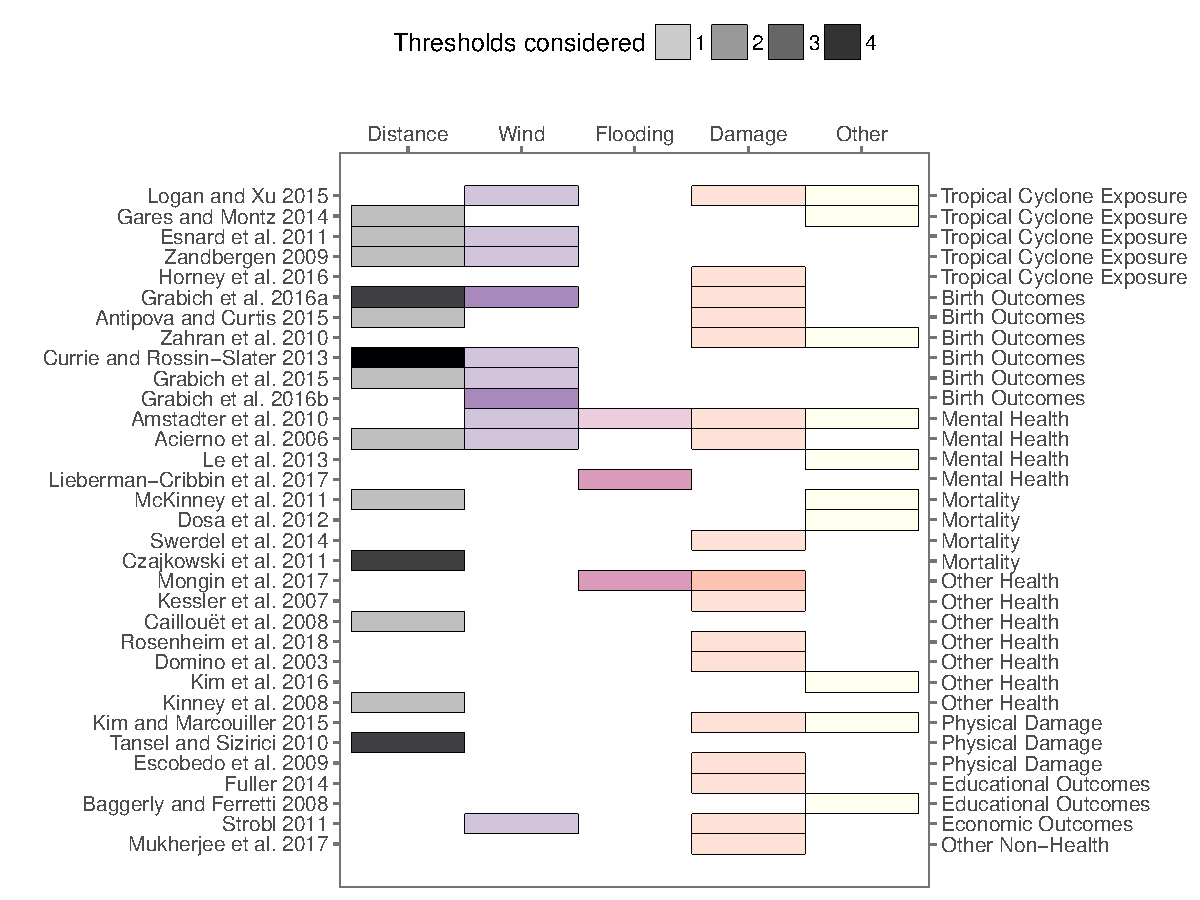
\includegraphics[width=\linewidth]{previous_exposure_metrics}
\caption{Metrics used in a sample of previous studies to assign exposure to
tropical cyclones in \ac{US}-based tropical cyclone exposure or impact studies.
Citations for each study are shown on the left and the broad topic of the study
on the left. Presence of a bar for a study-metric combination indicates that
the given metric was used in the study in assessing exposure to tropical
cyclones for that study, either alone or in combination with other metrics for
which that study has bars. The color transparency of each bar indicates the
number of different thresholds considered for defining storm exposure in the
study under that hazard (e.g., less transparent bars indicate that a study
considered multiple thresholds of the metric in defining tropical cyclone
exposure as a method of sensitivity analysis). Studies for which there are two
or more bars (e.g., bars for both distance and wind) indicate studies that
either used separate exposure assessments, one for each metric, (e.g., as a
sensitivity analysis) or used a single exposure index that incorporated
multiple metrics in its definition. ``Damage" often indicate use of Federal
Emergency Management Agency (FEMA) reports, although occasionally used damage
reports from other sources, including newspaper reports. Examples of ``Other"
include evacuation orders, excessive school closures, length of time a storm
was near a location, and detailed, holistic analyses of a specific storm or
storms. References for each study are included in the bibliography of this
Supplemental Material.}
\label{fig:previousmetrics}
\end{figure}

\nocite{logan2015, gares2014, esnard2011, zandbergen2009, horney2016,
grabich2016, antipova2015post, zahran2010, currie2013, grabich2015,
grabich2016hurricane, amstadter2010, acierno2006, le2013, lieberman2017,
mckinney2011, dosa2012evacuate, swerdel2014, czajkowski2011, mongin2017,
kessler2007hurricane, caillouet2008increase, rosenheim2018disaster,
domino2003disasters, kim2016, kinney2008, kim2015, tansel2010, escobedo2009,
fuller2014, baggerly2008impact, strobl2011economic, mukherjee2017}

\newpage

\end{comment}

\begin{figure}[tbhp!]
\centering
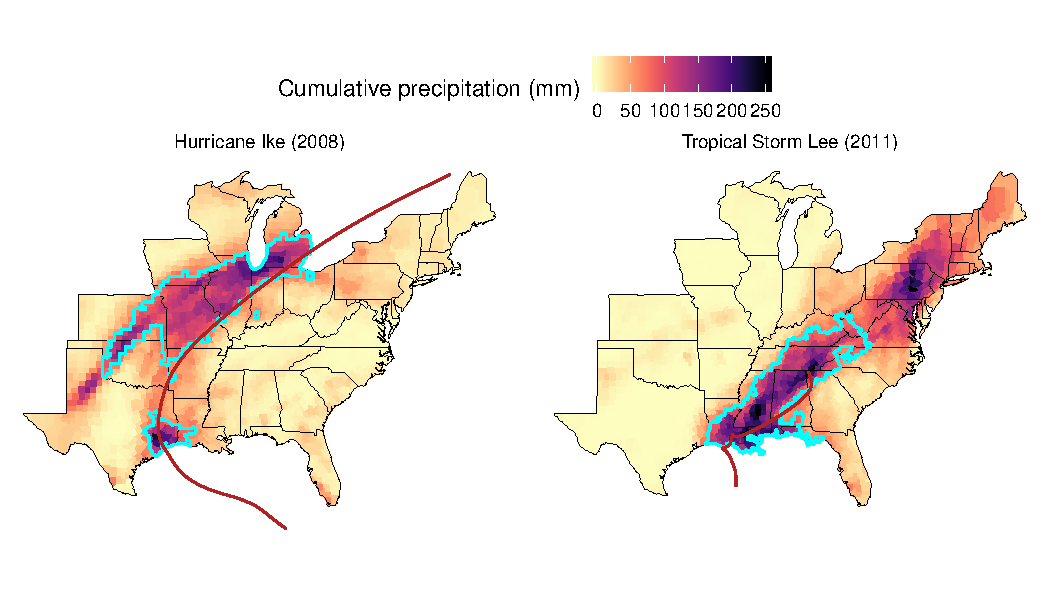
\includegraphics[width=0.9\linewidth]{rainexamples}
\caption{Examples of storms where some storm-related rainfall occured
         500 \si{\kilo\metre} or further from the storm's track. 
	 The red line on each map shows the track of the storm. 
	 The color of each county in the map gives the cumulative 
	 precipitation in the county from two days before to one day after
	 the storm's closest approach (in \si{\milli\metre}). The blue 
	 outline identifies the collection of counties
	 that were classified as ``exposed" based on the rainfall exposure 
	 criteria (Table 1 of main text), which includes the constraint
	 that the storm must have come within 500 \si{\kilo\metre} of the 
	 county. }
\label{fig:rainexamples}
\end{figure}

\clearpage 

\begin{figure}[tbhp!]
\centering
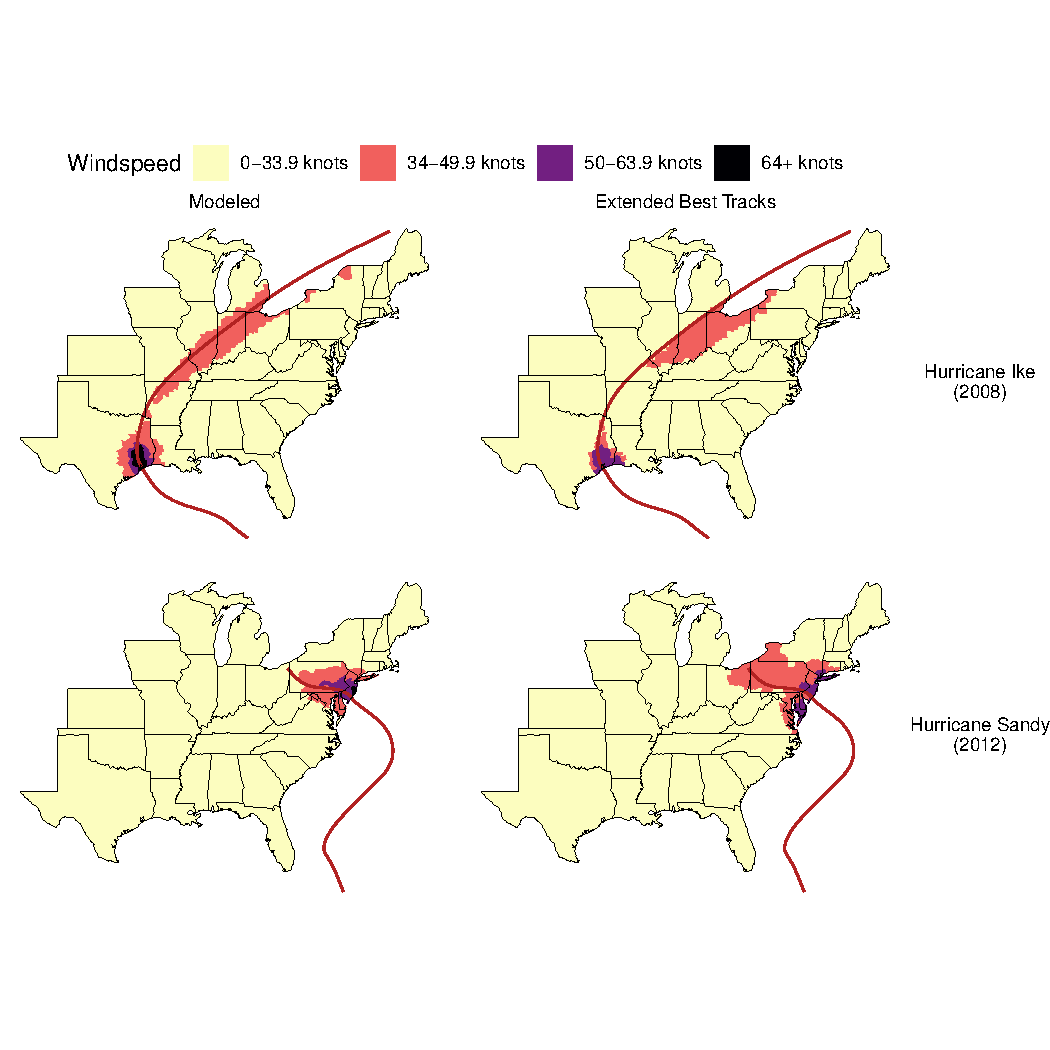
\includegraphics[width=\linewidth]{windexamples}
\caption{Comparison of county-level estimates of peak sustained surface wind 
	for Hurricane Ike in 2008 (top) and Hurriance Sandy in 2012 (bottom). 
	Each map shows the estimated peak sustained surface wind 
	classification ($<$34~kt; 34\,--\,49.9~kt; 
	50\,--\,63.9~kt; $\ge$64~kt) for each study county. 
	The maps labelled ``Modeled'' (left)
	shows the classifications based on modeled peak sustained surface wind,
	which were included in the open-source data as the main 
	wind metric and used in further analysis in this research. The maps
	labelled ``Extended Best Tracks'' (right) show classifications based on the 
	wind radii given in \ac{HURDAT2} (included as a secondary wind 
	metric in the open-source data). The red lines show the storms' 
	tracks.
	}
\label{fig:windexamples}
\end{figure}

\clearpage

\begin{figure}[tbhp!]
\centering
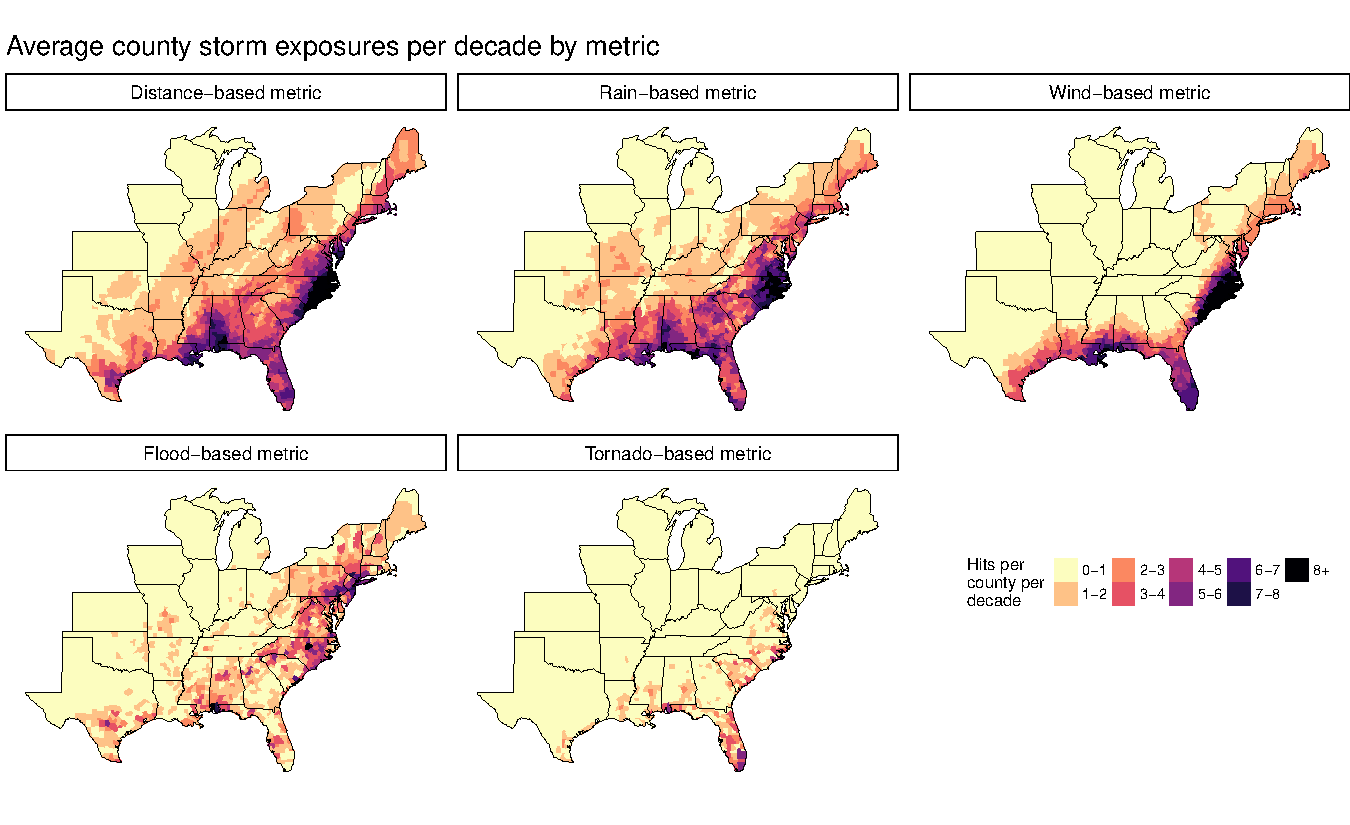
\includegraphics[width=7cm]{averageexposureonlysupp}
\caption{Average number of storm exposures per decade in U.S. counties for each 
	single-hazard exposure metric, limited analysis to years for which data on all five 
	exposures were available (1996\,--\,2011). The criteria behind each of 
	the five metrics is given in Table 1 of the main text. 	
	} 
\label{fig:averageexposuresupp}
\end{figure}

\clearpage 

\begin{figure}[tbhp!]
\centering
\includegraphics[width=\linewidth]{othertopstorms}
\caption{Differences in the counties assessed as ``exposed'', based on different
	exposure metrics, for a sample of storms. These sample storms were 
	selected as the  storms with largest extent (as measured by the 
	number of counties exposed based on any metric) from each of the 
	clusters shown in the Jaccard heatmap in the main text (Figure 7; a similar
	map for Hurricane Ivan in 2004 is shown in Figure 6 of the main text).}
\label{fig:othertopstorms}
\end{figure}

\clearpage

\begin{comment}

\begin{figure}[tbhp!]
\centering
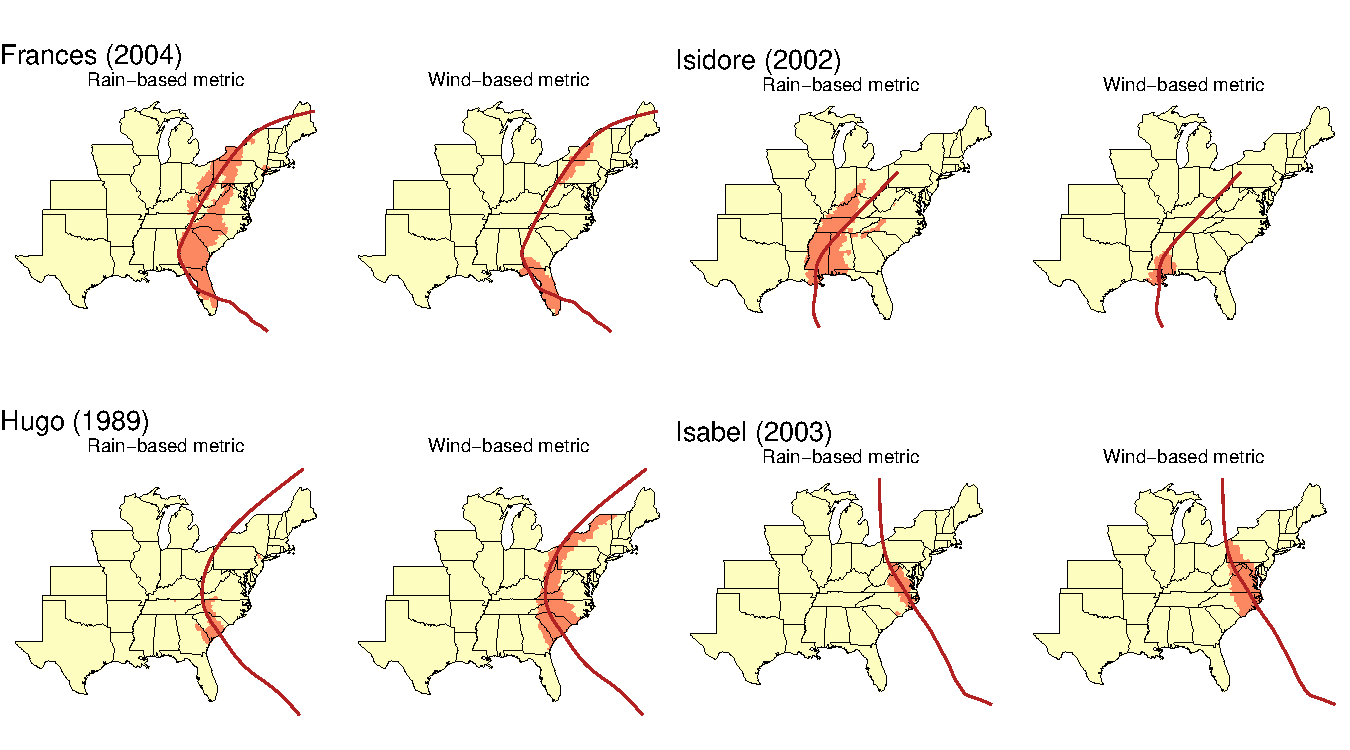
\includegraphics[width=\linewidth]{extentdisagreement}
\caption{Examples of storms for which exposure assessments differed
	substantially between rain-based and wind-based metrics. Counties 
	shown in orange were classified as exposed to a given storm by a 
	given metric; those in yellow were classified as not exposed. 
	The storm's track is shown in red. For both Frances (2004) and 
	Isidore (2002) (top panel), substantially more counties were assessed 
	as exposed when measuring exposure based on rain rather than wind. 
	Conversely, for both Hugo (1989) and Isabel (2003) (bottom panel), 
	substantially more counties were assessed as exposed based on wind 
	compared to rain.}
\label{fig:extentdisagreement}
\end{figure}

\clearpage

\end{comment}

\begin{longtable}{lp{40em}}
\caption{Caption. These are provided for the three exposure metrics for which our database includes continuous data, and so a threshold is selected to determine binary exposure based on the metric. This table provides reasoning for the choice of threshold used in this paper as well as guidance on other thresholds that could be considered, depending on the hypothesized pathways for an epidemiological study.}
\label{tab:thresholds} \\
\hline
Metric & Threshold choice\\
\hline
Distance & In the manuscript, distance-based exposure was assessed if the storm track came within 100 km of county population mean center. This threshold for distance from the storm center has been used in prior research as a proxy for exposure to hazards from the storm \parencite{grabich2015measuring}. Tropical cyclones vary dramatically in size: US tropical cyclones have been observed with radii to maximum winds as small as 20 km and as large as 200 km \parencite{mallin2006, quiring2011variations}, and dangerous winds can extend beyond these maximum winds. One study \parencite{czajkowski2011} assessed county-level risk and exposure based on a three-tiered definition, with primary counties being those closest to the storm track on either side, secondary counties being adjacent to primary counties, and tertiary counties adjacent to secondary counties. Such a definition resulted in an exposure defenition based on an average distance radius of 120 km on either side of the storm track \parencite{czajkowski2011}. Other distance thresholds that could be considered include 60 km and 30 km, both of which have been used in previous research \parencite{grabich2015measuring, grabich2015, currie2013}.\\
Rain & In the manuscript, rain-based exposure was assessed if the county had cumulative rainfall of $\ge75$ mm over the period from two days before to one day after the storm’s closest approach and the storm track came within 500 km of the county population mean center. This threshold... Other reasonable definitions could vary both the threshold of rainfall (in mm) and also the choice of days surrounding the storm to include when calculating the cumulative rainfall. Tropical cyclone precipitation arrives before the center of the storm \parencite{zhou2017spatial}. A variety of definitions have been used to identify both extreme or heavy rain (whether associated with a tropical cyclone or not) and tropical cyclone--associated rain. Some definitions of extreme rain events are higher than the threshold we use here---for example, one paper defined extreme rain events as cases in which a gauge reported 125 mm or more of rain in 24 hours \parencite{schumacher2006characteristics}. Studies have also used definitions that are relative to the norms for a given location (e.g., 24 hour rainfall totals over the 50-year return value for the location, which the part of the US east of the Rocky Mountains range from 3.5 in [89 mm] to 13 in [330 mm]). \parencite{schumacher2006characteristics, schumacher2005organization, stevenson201410}. A study focused on the risks that result from extreme rainfall may therefore reasonably choose a higher threshold than the 75 mm threshold we use in this analysis. In defining precipitation associated with tropical cyclones, studies have used thresholds of 12.5 mm per day as a metric of regions of ``moderately heavy'' rainfall \parencite{zhou2017spatial} and, as a lower threshold, a lower limit of 10 mm of total storm precipitation---in conjunction with proximity to the storm's center---in identifying tropical cyclone precipitation events at a location \parencite{feldmann2019estimation}. \\
Wind & In the manuscript, wind-based exposure was assessed if modeled storm-associated peak sustained surface wind of $\ge34$ kts at the county’s population mean center. This threshold is being applied to local winds for each county, and it represents the threshold for gale-force winds on the Beaufort wind scale. This limit is used as the outer limit in measuring storm size through the US National Hurricane Center's wind radii for tropical cyclone forecasts \parencite{cangialosi2016examination}. Other thresholds could be selected based on other points on the Beaufort scale---for example, $\ge48$ kts for capturing storm-force winds or $\ge64$ kts for capturing hurricane-force winds. As a note, hurricane-force winds will be rarely experienced for counties, as it will likely only be observed for very severe storms and even for those for counties near the storm's landfall. Many presentations of the Beaufort wind scale include descriptions of the conditions that winds in each category would produce both over land and at sea.\\
\hline
\end{longtable}

\clearpage

\begin{table}

\caption{\label{tab:highprecipcorr}Precipitation correlation during all versus high-precipitation events.
                     The same sample of counties is shown as in Figure 2 of the main text.
                     Events are cases where a tropical cyclone came within 500 km of each of the 
                     listed counties. The number of total events gives the sum of all points
                     shown on the main plot for the county in Figure 2 of the main text. 
                     The Spearman correlation for all events is the same as that shown in Figure 2
                     of the main text. High-precipitation events are those for which storm-associated
                     precipitation was 75 mm or higher based on at least one of the two measures
                     considered in this comparison (NLDAS-2 reanalysis data and ground-based stations). The Spearman correlation between these two precipitation data sources is given
                     for these high-precipitation events in the last column of the 
                     table.}
\centering
\begin{tabular}[t]{lcccc}
\toprule
\multicolumn{1}{c}{ } & \multicolumn{2}{c}{All events} & \multicolumn{2}{c}{High-precipitation events} \\
\cmidrule(l{3pt}r{3pt}){2-3} \cmidrule(l{3pt}r{3pt}){4-5}
County & \makecell[c]{Number\\of events} & \makecell[c]{Spearman\\correlation} & \makecell[c]{Number\\of events} & \makecell[c]{Spearman\\correlation}\\
\midrule
Miami-Dade, FL & 65 & 0.94 & 18 & 0.49\\
Harris, TX & 38 & 0.93 & 10 & 0.84\\
Mobile, AL & 50 & 0.95 & 20 & 0.57\\
Orleans, LA & 55 & 0.89 & 13 & 0.95\\
Fulton, GA & 48 & 0.95 & 12 & 0.69\\
\addlinespace
Charleston, SC & 73 & 0.94 & 17 & 0.65\\
Wake, NC & 61 & 0.98 & 12 & 0.84\\
Baltimore, MD & 33 & 0.92 & 5 & 0.70\\
Philadelphia, PA & 52 & 0.96 & 6 & 0.77\\
\bottomrule
\end{tabular}
\end{table}


\clearpage

% latex table generated in R 4.0.2 by xtable 1.8-4 package
% Tue Sep  1 17:11:57 2020
\begin{table}[ht]
\centering
\caption{Caption. Limited to storms with at least 200 counties assessed as exposed based on at least one exposure metric considered in this study. Numbers are out of 2,396 counties in the study area (states in the eastern half of the US). Exposure assessment is based on the thresholds given in Table 1 of the main text. The Jaccard index shown in Figure [x] of the main text is based on numbers in the second through fourth columns (the value in the second column divide by the sum of numbers in the second through fourth columns). Storms are ordered based on the number of counties exposed to at least one of these two exposure metrics.} 
\begin{tabular}{cp{3cm}p{3cm}p{3cm}p{3cm}}
  \toprule
Storm & Classified as exposed based on both distance metric and wind metric & Classified as exposed based on distance metric but unexposed by wind metric & Classified as exposed based on wind metric but unexposed by distance metric & Classified as unexposed based on both distance metric and wind metric \\ 
  \midrule
Frances-2004 &  44 & 277 &  13 & 2062 \\ 
  Cindy-2005 &  17 & 304 &   4 & 2071 \\ 
  Dennis-2005 &  18 & 274 &  26 & 2078 \\ 
  Ike-2008 & 166 &  67 &  82 & 2081 \\ 
  Ivan-2004 &  29 & 255 &  27 & 2085 \\ 
  Jeanne-2004 &  41 & 256 &   7 & 2092 \\ 
  Allison-2001 &  21 & 266 &   0 & 2109 \\ 
  Isidore-2002 &  29 & 239 &   7 & 2121 \\ 
  Katrina-2005 &  66 & 175 &  32 & 2123 \\ 
  Gordon-2000 &  11 & 244 &   6 & 2135 \\ 
  Fay-2008 &  54 & 198 &   7 & 2137 \\ 
  Gustav-2008 &  36 & 198 &  23 & 2139 \\ 
  Bertha-1996 & 179 &   4 &  62 & 2151 \\ 
  Danny-1997 &  45 & 184 &  12 & 2155 \\ 
  Arlene-2005 &   4 & 232 &   0 & 2160 \\ 
  Bill-2003 &  19 & 211 &   0 & 2166 \\ 
  Dennis-1999 &  17 & 183 &  13 & 2183 \\ 
  Hanna-2008 & 135 &  57 &  12 & 2192 \\ 
  Isabel-2003 & 105 &  42 &  56 & 2193 \\ 
  Ernesto-2006 &  93 &  99 &   4 & 2200 \\ 
  Helene-2000 &  18 & 174 &   0 & 2204 \\ 
  Rita-2005 &  26 & 139 &  20 & 2211 \\ 
  Fran-1996 &  46 & 105 &  30 & 2215 \\ 
  Earl-1998 & 133 &  36 &  11 & 2216 \\ 
  Floyd-1999 & 124 &  15 &  40 & 2217 \\ 
  Irene-2011 & 114 &   6 &  46 & 2230 \\ 
  Lee-2011 &  34 & 110 &   0 & 2252 \\ 
  Josephine-1996 &  62 &  61 &   3 & 2270 \\ 
  Hermine-2010 &  22 & 101 &   1 & 2272 \\ 
  Bonnie-2004 &   0 & 109 &   0 & 2287 \\ 
  Frances-1998 &  15 &  47 &   0 & 2334 \\ 
   \bottomrule
\end{tabular}
\end{table}


\clearpage

% latex table generated in R 4.0.2 by xtable 1.8-4 package
% Tue Sep  1 16:45:11 2020
 & storm\_id & dist\_rain & dist\_no\_rain & no\_dist\_rain & neither \\ 
  \midrule
1 & Frances-2004 & 207 & 114 & 257 & 1818 \\ 
  2 & Ivan-2004 & 124 & 160 & 288 & 1824 \\ 
  3 & Isidore-2002 & 134 & 134 & 186 & 1942 \\ 
  4 & Ike-2008 & 113 & 120 & 213 & 1950 \\ 
  5 & Dennis-2005 &  48 & 244 & 124 & 1980 \\ 
  6 & Fay-2008 &  72 & 180 & 163 & 1981 \\ 
  7 & Jeanne-2004 & 144 & 153 & 113 & 1986 \\ 
  8 & Lee-2011 & 106 &  38 & 230 & 2022 \\ 
  9 & Gustav-2008 & 126 & 108 & 137 & 2025 \\ 
  10 & Allison-2001 & 106 & 181 &  67 & 2042 \\ 
  11 & Bill-2003 & 110 & 120 & 117 & 2049 \\ 
  12 & Cindy-2005 &  78 & 243 &  11 & 2064 \\ 
  13 & Floyd-1999 & 129 &  10 & 170 & 2087 \\ 
  14 & Katrina-2005 & 195 &  46 &  58 & 2097 \\ 
  15 & Danny-1997 &  82 & 147 &  54 & 2113 \\ 
  16 & Rita-2005 &  64 & 101 & 103 & 2128 \\ 
  17 & Gordon-2000 &   5 & 250 &   7 & 2134 \\ 
  18 & Arlene-2005 &  39 & 197 &  23 & 2137 \\ 
  19 & Dennis-1999 &  90 & 110 &  56 & 2140 \\ 
  20 & Ernesto-2006 & 124 &  68 &  63 & 2141 \\ 
  21 & Irene-2011 & 119 &   1 & 106 & 2170 \\ 
  22 & Hanna-2008 & 100 &  92 &  33 & 2171 \\ 
  23 & Hermine-2010 &  44 &  79 & 102 & 2171 \\ 
  24 & Fran-1996 &  89 &  62 &  73 & 2172 \\ 
  25 & Earl-1998 &  72 &  97 &  38 & 2189 \\ 
  26 & Bertha-1996 & 103 &  80 &  20 & 2193 \\ 
  27 & Helene-2000 &  28 & 164 &  11 & 2193 \\ 
  28 & Frances-1998 &  27 &  35 & 139 & 2195 \\ 
  29 & Josephine-1996 &  94 &  29 &  77 & 2196 \\ 
  30 & Tammy-2005 &  12 &  90 &  97 & 2197 \\ 
  31 & Alberto-2006 &  72 &  77 &  40 & 2207 \\ 
  32 & Bonnie-2004 &  56 &  53 &  56 & 2231 \\ 
  33 & Barry-2007 &  39 &  87 &  38 & 2232 \\ 
  34 & Isabel-2003 &  88 &  59 &  17 & 2232 \\ 
  35 & Hanna-2002 &   6 &  60 &  97 & 2233 \\ 
  36 & Ida-2009 &  10 &  20 & 132 & 2234 \\ 
  37 & Charley-2004 &  77 &  46 &  36 & 2237 \\ 
  38 & Erin-2007 &  44 &  69 &  31 & 2252 \\ 
  39 & Five-2010 &   6 & 125 &  11 & 2254 \\ 
  40 & Barry-2001 &   7 & 119 &   9 & 2261 \\ 
  41 & Georges-1998 &  69 &  15 &  44 & 2268 \\ 
  42 & Grace-2003 &   9 &  64 &  54 & 2269 \\ 
  43 & Kyle-2002 &  10 &  39 &  77 & 2270 \\ 
  44 & Gaston-2004 &  45 &  65 &   0 & 2286 \\ 
  45 & Lili-2002 &  19 &  71 &  19 & 2287 \\ 
  46 & Matthew-2004 &  67 &   5 &  31 & 2293 \\ 
   \bottomrule


\clearpage

% latex table generated in R 4.0.2 by xtable 1.8-4 package
% Wed Sep  9 14:27:55 2020
\begin{table}[ht]
\centering
\caption{Caption. Limited to storms with at least 250 counties assessed as exposed based on at least one exposure metric considered in this study. Numbers are out of 2,396 counties in the study area (states in the eastern half of the US). Exposure assessment is based on the thresholds given in Table 1 of the main text. The Jaccard index shown in Figure [x] of the main text is based on numbers in the second through fourth columns (the value in the second column divide by the sum of numbers in the second through fourth columns). Storms are ordered based on the number of counties exposed to at least one of these two exposure metrics.} 
\label{tab:misclassflood}
\begin{tabular}{cp{3cm}p{3cm}p{3cm}p{3cm}}
  \toprule
Storm & Exposed for both distance metric and flood metric & Exposed for distance metric but unexposed for flood metric & Exposed for flood metric but unexposed for distance metric & Unexposed for both distance metric and flood metric \\ 
  \midrule
Ivan (2004) & 79 & 205 & 238 & 1,874 \\ 
  Frances (2004) & 103 & 218 & 122 & 1,953 \\ 
  Dennis (2005) & 21 & 271 & 87 & 2,017 \\ 
  Jeanne (2004) & 80 & 217 & 77 & 2,022 \\ 
  Allison (2001) & 68 & 219 & 71 & 2,038 \\ 
  Cindy (2005) & 52 & 269 & 29 & 2,046 \\ 
  Ike (2008) & 48 & 185 & 101 & 2,062 \\ 
  Isidore (2002) & 30 & 238 & 64 & 2,064 \\ 
  Fay (2008) & 23 & 229 & 60 & 2,084 \\ 
  Bill (2003) & 39 & 191 & 65 & 2,101 \\ 
  Gustav (2008) & 36 & 198 & 57 & 2,105 \\ 
  Katrina (2005) & 47 & 194 & 47 & 2,108 \\ 
  Gordon (2000) & 7 & 248 & 19 & 2,122 \\ 
  Arlene (2005) & 11 & 225 & 29 & 2,131 \\ 
  Danny (1997) & 39 & 190 & 31 & 2,136 \\ 
  Floyd (1999) & 100 & 39 & 120 & 2,137 \\ 
  Fran (1996) & 46 & 105 & 77 & 2,168 \\ 
  Dennis (1999) & 38 & 162 & 19 & 2,177 \\ 
  Ernesto (2006) & 44 & 148 & 27 & 2,177 \\ 
  Bertha (1996) & 27 & 156 & 17 & 2,196 \\ 
  Rita (2005) & 4 & 161 & 26 & 2,205 \\ 
  Lee (2011) & 18 & 126 & 36 & 2,216 \\ 
   \bottomrule
\end{tabular}
\end{table}


\clearpage

% latex table generated in R 4.0.2 by xtable 1.8-4 package
% Thu Sep  3 12:19:54 2020
\begin{table}[ht]
\centering
\caption{Caption. Limited to storms with at least 250 counties assessed as exposed based on at least one exposure metric considered in this study. Numbers are out of 2,396 counties in the study area (states in the eastern half of the US). Exposure assessment is based on the thresholds given in Table 1 of the main text. The Jaccard index shown in Figure [x] of the main text is based on numbers in the second through fourth columns (the value in the second column divide by the sum of numbers in the second through fourth columns). Storms are ordered based on the number of counties exposed to at least one of these two exposure metrics.} 
\begin{tabular}{cp{3cm}p{3cm}p{3cm}p{3cm}}
  \toprule
Storm & Exposed for both distance metric and tornado metric & Exposed for distance metric but unexposed for tornado metric & Exposed for tornado metric but unexposed for distance metric & Unexposed for both distance metric and tornado metric \\ 
  \midrule
Frances (2004) & 6 & 315 & 66 & 2,009 \\ 
  Ivan (2004) & 36 & 248 & 55 & 2,057 \\ 
  Cindy (2005) & 27 & 294 & 11 & 2,064 \\ 
  Jeanne (2004) & 13 & 284 & 22 & 2,077 \\ 
  Dennis (2005) & 0 & 292 & 6 & 2,098 \\ 
  Allison (2001) & 14 & 273 & 9 & 2,100 \\ 
  Katrina (2005) & 8 & 233 & 38 & 2,117 \\ 
  Fay (2008) & 15 & 237 & 26 & 2,118 \\ 
  Isidore (2002) & 1 & 267 & 6 & 2,122 \\ 
  Ike (2008) & 4 & 229 & 31 & 2,132 \\ 
  Gordon (2000) & 1 & 254 & 8 & 2,133 \\ 
  Gustav (2008) & 9 & 225 & 28 & 2,134 \\ 
  Bill (2003) & 4 & 226 & 22 & 2,144 \\ 
  Arlene (2005) & 2 & 234 & 7 & 2,153 \\ 
  Danny (1997) & 9 & 220 & 4 & 2,163 \\ 
  Rita (2005) & 8 & 157 & 41 & 2,190 \\ 
  Dennis (1999) & 0 & 200 & 1 & 2,195 \\ 
  Ernesto (2006) & 2 & 190 & 1 & 2,203 \\ 
  Bertha (1996) & 13 & 170 & 4 & 2,209 \\ 
  Fran (1996) & 1 & 150 & 4 & 2,241 \\ 
  Lee (2011) & 14 & 130 & 11 & 2,241 \\ 
  Floyd (1999) & 11 & 128 & 1 & 2,256 \\ 
   \bottomrule
\end{tabular}
\end{table}


\clearpage

\printbibliography

\end{document}

